\documentclass[10pt,letterpaper]{article}
\usepackage[hang,flushmargin]{footmisc}
\usepackage[latin1]{inputenc}
\usepackage[letterpaper,margin=1in]{geometry}
\usepackage{amsfonts}
\usepackage{amsmath}
\usepackage{amsmath}
\usepackage{amssymb}
\usepackage{bm}
\usepackage{booktabs}
\usepackage[labelfont=bf]{caption}
\usepackage{graphicx}
\usepackage{mathtools}
\usepackage{minted}
\usepackage{parskip}
\usepackage{subcaption}
\usepackage{url}
\usepackage{xcolor}
\numberwithin{figure}{section}
\numberwithin{table}{section}

\definecolor{bg}{rgb}{0.90,0.90,0.910}
\DeclarePairedDelimiterX\set[1]\lbrace\rbrace{\def\given{\;\delimsize\vert\;}#1}

\author{fsaad}
\title{Compositional Metamodeling Language}

\begin{document}
\maketitle

\section{Populations, Variables, and Measurement Types}
\label{sec:populations-measurements}

The Metamodeling Language formalizes the notion of a
\textit{statistical population} to be a collection of named variables,
$\bm{X} = \set{X_1,\dots,X_D}$. Each variable $X_i$ takes values in a
measurement space $\mathcal{X}_i$, known to MML only through a qualitative
token called the \textit{measurement type}.

Some possible measurement types and associated spaces $\mathcal{X}$ for
population variables are shown in Table \ref{tab:measurement-types}.

\begin{table}[h]
\centering
\begin{tabular}{@{}ll@{}}
    \toprule
    Measurement Type & Example Measurement Spaces\\ \midrule
    Audio & $\set{0,1}^4$, pulse code modulated signals.\\
    Binary & $\{0,1$\}, \{boy, girl\}, any arbitrary binary labels.\\
    Circular & $(-\pi, \pi]$, wall clock, directional sets that can be
        ``wrapped".\\
    Counts & $\{0,1,2,\dots\}$, frequencies, rates.\\
    Categorical & $\{1,\dots,K\}$, finite unordered sets with arbitrary labels.\\
    Image & \begin{tabular}[c]{@{}l@{}}
        URL i.e \url{http://fsaad.mit.edu/media/mypic.jpg}, or \\
        pixel matrices $\set{0,1}^{28\times28}$.\end{tabular} \\
    Numerical & $\mathbb{R}, [0, 100]$, uncountable sets.\\
    Ordinal & \{`small',`medium',`large'\}, finite well-ordered set with arbitrary labels.\\
    \bottomrule
\end{tabular}
\caption{Possible measurement types for the variables in a population.
    These measurement types and spaces are not comprehensive, and not all are
    implemented in MML.}
\label{tab:measurement-types}
\end{table}

Populations in MML are declared using \texttt{CREATE POPULATION}, followed by a
\textit{population schema}
\footnote{The \texttt{swallow} population will be used as a running example in
this document. This dataset is collected from an ecology experiment that studied
the orientation of juvenile barn swallows (birds) under two magnetic field
treatments, local and shifted. The research question was whether swallows can
use magnetic information for compass orientation \cite{Giunchi2004}.}.

\begin{minted}
[bgcolor=bg,framesep=2mm,baselinestretch=1.2,fontsize=\footnotesize,linenos]{sql}
CREATE POPULATION swallows(
    treatment BINARY,
    orientation CIRCULAR(0, 6.28));
\end{minted}

The variables in the \texttt{swallows} population are \texttt{treatment} and
\texttt{orientation}, and their measurement types are \texttt{BINARY} and
\texttt{CIRCULAR}.

A \textit{member} of the population is a measurement $\bm{x}_i$, which is a
multivariate entity with $D$ attributes. Entry $x_{ij}$ takes values in the
measurement space $\mathcal{X}_j$ of the $j$th variable declared in the
population schema. Members of a population have neither probabilistic
interpretations nor any distributional assumptions.

MML \texttt{INCORPORATE} loads measurements into a population from a data
source. Every incorporated measurement is implicitly assigned a binary
\texttt{primary key} (or \texttt{pk}) by MML, which is a unique identifier for
all measurements across all populations.

\begin{minted}
[bgcolor=bg,framesep=2mm,baselinestretch=1.2,fontsize=\footnotesize,linenos]{sql}
INCORPORATE INTO swallows OBSERVATIONS swallows.csv
\end{minted}

The first 5 measurements can be viewed using a SQL query.

\begin{minted}
[bgcolor=bg,framesep=2mm,baselinestretch=1.2,fontsize=\footnotesize,linenos]{sql}
SELECT * FROM swallows LIMIT 5
\end{minted}

\begin{table}[h]
\centering
\begin{tabular}{@{}ll@{}}
\toprule
\textbf{treatment} & \textbf{orientation} \\ \midrule
local & 5.38 \\
local & 2.32 \\
shifted & 3.63 \\
local & 0.28 \\ \bottomrule
\end{tabular}
\label{tab:bql-select}
\caption{Five measurements from the \texttt{swallows} population. The
measurement space for the \texttt{BINARY} variable \texttt{treatment} is
\{`local', shifted\}, and for \texttt{orientation} is $[0,2\pi)$.}
\end{table}

\section{Schemas for Generative Population Models}

In Section \ref{sec:populations-measurements} it was explained that a population
is not associated with any particular model, it is merely a collection of
measurements. The contents of a population can be queried using languages such
as SQL.

A \textit{generative population model} (GPM) encodes modeling assumptions for
the measurement-generating process of variables in populations. From the
perspective of MML, a GPM is a \textit{procedure} which can

\begin{itemize}
\item \texttt{GENERATE} measurements of (a sub-collection of) variables from
some population,
\item be \texttt{GIVEN} measurements of other variables in the population that
it needs to generate its outputs,
\item use a \texttt{PROGRAM}, opaque to MML, that contains modeling commands.
\end{itemize}

GPMs offer a form of procedural abstraction for probabilistic and non-
probabilistic models. MML cannot see inside the \texttt{PROGRAM} of a GPM. The
behavior of the GPM is only known to MML in terms of the \texttt{GENERATE} and
\texttt{GIVEN} variables.

\textbf{Instances of} GPMs in MML are declared using \texttt{CREATE GPM},
followed by a \textit{schema}

\begin{minted}
[bgcolor=bg,framesep=2mm,baselinestretch=1.2,fontsize=\footnotesize,linenos]{sql}
CREATE GPM treat-bernoulli FOR swallows USING bernoulli(
    GENERATE (treatment)
    GIVEN (NULL)
    PROGRAM (prior beta(1,1))
\end{minted}

The \texttt{treat-bernoulli} GPM is a density estimator for the marginal
distribution of the \texttt{treatment} variable. As an
\textit{instance} of the \texttt{bernoulli} GPM\footnote{A good question is
``where did \texttt{bernoulli} GPM come from?" It was compiled with MML.},
\texttt{treat-bernoulli} assumes that measurements of \texttt{treatment} are
observations from an exchangeable sequence of Bernoulli flips with weight
$\theta$. The \texttt{bernoulli} GPM can only accept one variable in
\texttt{GENERATE} whose measurement type is \texttt{BINARY}.

\texttt{GIVEN} is empty since no other variables are needed to generate
measurements from this marginal distribution. The \texttt{PROGRAM} is a binary
opaque to MML. In this instance, \texttt{bernoulli} allows modeling
commands to specify the prior over weight $\theta$. Every GPM has its
own parser for the contents of \texttt{PROGRAM}. Another schema that
\texttt{bernoulli} would accept is

\begin{minted}
[bgcolor=bg,framesep=2mm,baselinestretch=1.2,fontsize=\footnotesize,linenos]{sql}
CREATE GPM ... USING bernoulli (
    ...
    PROGRAM (maximum-likelihood))
\end{minted}

MML allows users to \texttt{INITIALIZE} multiple independent instances of a GPM
with the same schema. This strategy is usually desirable for complex GPMs which
have a high degree of uncertainty in their own generative processes.

\begin{minted}
[bgcolor=bg,framesep=2mm,baselinestretch=1.2,fontsize=\footnotesize,linenos]{sql}
INITIALIZE 2 INSTANCES OF treat-bernoulli
\end{minted}

\section{Modeling Directives for Generative Population Models}

The \texttt{INCORPORATE} command must be used explicitly to load measurements
into a GPM\footnote{This strategy allows GPMs to observe/unobserve and perform
other dynamic inference controls, without having to worry about manipulating the
data directly in the population and interfering with other GPMs on the same
population. The population is just a data store. This strategy also allows
different GPMs over the same variables to observe different measurements
(subsampling)}.

\begin{minted}
[bgcolor=bg,framesep=2mm,baselinestretch=1.2,fontsize=\footnotesize,linenos]{sql}
INCORPORATE INTO treat-bernoulli OBSERVATIONS (
    SELECT treatment FROM swallows WHERE pk <= 5)
\end{minted}

Since the GPM generates variable \texttt{swallows.treatment}, every incorporated
measurement must have a corresponding primary key in the \texttt{swallows}
population. The previous example only incorporated the first five measurements
from \texttt{swallows}. \texttt{treat-bernoulli} can reveal which measurements
have been incorporated.

\begin{minted}
[bgcolor=bg,framesep=2mm,baselinestretch=1.2,fontsize=\footnotesize,linenos]{sql}
SELECT pk FROM treat-bernoulli
\end{minted}

\begin{table}[!htbp]
\centering
\begin{tabular}{@{}ll@{}}
\toprule
\textbf{treat-bernoulli.pk} \\ \midrule
swallows.\#1 \\
swallows.\#2 \\
swallows.\#3 \\
swallows.\#4 \\
swallows.\#5 \\ \bottomrule
\end{tabular}
\label{tab:bql-pks}
\caption{Primary keys of observations incorporated into the
\texttt{treat-bernoulli} GPM.}
\end{table}

MML also permits \texttt{UNINCORPORATE} of observations\footnote{
Unincorporating an observation with a \texttt{pk} that has not been incorporated
will be ignored, or raise, or warn, etc.}.

\begin{minted}
[bgcolor=bg,framesep=2mm,baselinestretch=1.2,fontsize=\footnotesize,linenos]{sql}
UNINCORPORATE FROM treat-bernoulli OBSERVATIONS (
    SELECT treatment FROM swallows WHERE treatment = 'local')
\end{minted}

Unincorporating only some variables $x_{ij}$ from a member $\bm{x_i}$ is
supported. A primary key is unincorporated from a GPM once all its variables
have been unincorporated.

Multiple GPMs can be created for the same population variable. For instance, the
\texttt{frequency} GPM is a much simpler density estimator for
\texttt{treatment}. It learns a distribution by counting the empirical
frequencies of all its incorporated measurements, and takes no program.

\begin{minted}
[bgcolor=bg,framesep=2mm,baselinestretch=1.2,fontsize=\footnotesize,linenos]{sql}
CREATE GPM swallow-freq USING frequency(
    GENERATE (treatment) GIVEN (NULL) PROGRAM (NULL)
-- Incorporate all the treatment data.
INCORPORATE INTO swallow-freq OBSERVATIONS (SELECT treatment FROM swallows)
\end{minted}

An important point. The \texttt{frequency} GPM is applicable to variables
of any \textit{measurement type} (Table \ref{tab:measurement-types}), since it
only tallies frequencies of occurrences. It can also accept several variables in
\texttt{GENERATE} and learns joint distributions by counting joint frequencies
of observations.

MML can instruct swallow-freq to \texttt{UPDATE SCHEMA} to also model the
\texttt{orientation} variable.

\begin{minted}
[bgcolor=bg,framesep=2mm,baselinestretch=1.2,fontsize=\footnotesize,linenos]{sql}
UPDATE SCHEMA FOR swallow-freq(GENERATE (orientation))
\end{minted}

Since the \texttt{GIVEN} and \texttt{PROGRAM} are both \texttt{NULL}, they have
been omitted. Without \texttt{INCORPORATE}, however, the \texttt{swallow-freq}
GPM has missing data for all the \texttt{orientation} variables.

\begin{minted}
[bgcolor=bg,framesep=2mm,baselinestretch=1.2,fontsize=\footnotesize,linenos]{sql}
INCORPORATE INTO swallow-freq OBSERVATIONS(
    SELECT orientation FROM swallows WHERE pk <= 10)
\end{minted}

Only the first 10 observations in \texttt{swallow-freq} have complete
data now. The rest have observations only for the \texttt{treatment}
variable. Using \texttt{frequency} GPM for \texttt{NUMERICAL} data is rarely a
good idea.

\section{Inference Directives for Generative Population Models}

After incorporating data into a GPM, it can now learn more about its generative
process, a process called \textit{learning} or \textit{posterior inference}.
MML instructs the GPM to \texttt{ANALYZE}, optionally taking a
\texttt{PROGRAM}.

\begin{minted}
[bgcolor=bg,framesep=2mm,baselinestretch=1.2,fontsize=\footnotesize,linenos]{sql}
ANALYZE swallow-freq(
    TIMEOUT = 100s)
\end{minted}

After \texttt{ANALYZE} has completed, \texttt{swallow-freq} will recompute the
frequency table for outcomes of its variables, which jointly take values
in the product space \{`local',`shifted'\} $\times [0, 2\pi)$. The code
(\texttt{TIMEOUT = 100s}) is a program, opaque to MML, which tells the GPM to time out
after 100 seconds (ie if the frequency table is very large). More elaborate
programs will be encountered next.

\section{Review of Metamodeling Directives}

MML is a very small language. Its power comes from the fact that it is
\textit{extensible}. The key language constructs are

\begin{minted}
[bgcolor=bg,framesep=2mm,baselinestretch=1.2,fontsize=\footnotesize,linenos]{sql}
CREATE POPULATION <pop-name> (
    <variable> <measurement-type>[, ...])

CREATE GPM <gpm-name> FOR <pop-name> USING <gpm>(
    GENERATE (<variables> [, ...])
    [GIVEN (<variables> [, ...])]
    PROGRAM ([<blob>])
)

INITIALIZE <k> INSTANCES OF <gpm-name>

INCORPORATE INTO <pop|gpm> OBSERVATIONS <data-source>
UNINCORPORATE FROM <pop|gpm> OBSERVATIONS <data-source>

UPDATE SCHEMA FOR <gpm> (
    [GENERATE (<variables> [, ...])]
    [GIVEN (<variables> [, ...])]
    ([<program>])
)

ANALYZE <gpm> ([<program>])
\end{minted}

The full set of invariants and constraints that govern rules for the MML
directives is left for a separate technical document. One quick example is that,
for a GPM with \texttt{GIVEN} variables, every incorporated measurement must
include fully observed data for those variables. Many other rules relating to
primary key constraints, etc, exist.

\section{Compositional Metamodeling}

The running example of the \texttt{swallows} population
will be investigated further. Figure \ref{fig:histogram} shows the data to be
modeled. The illustration will proceed by incrementally building more complex
probabilistic models using simple primitives in the metamodeling language.

\begin{figure}[ht]
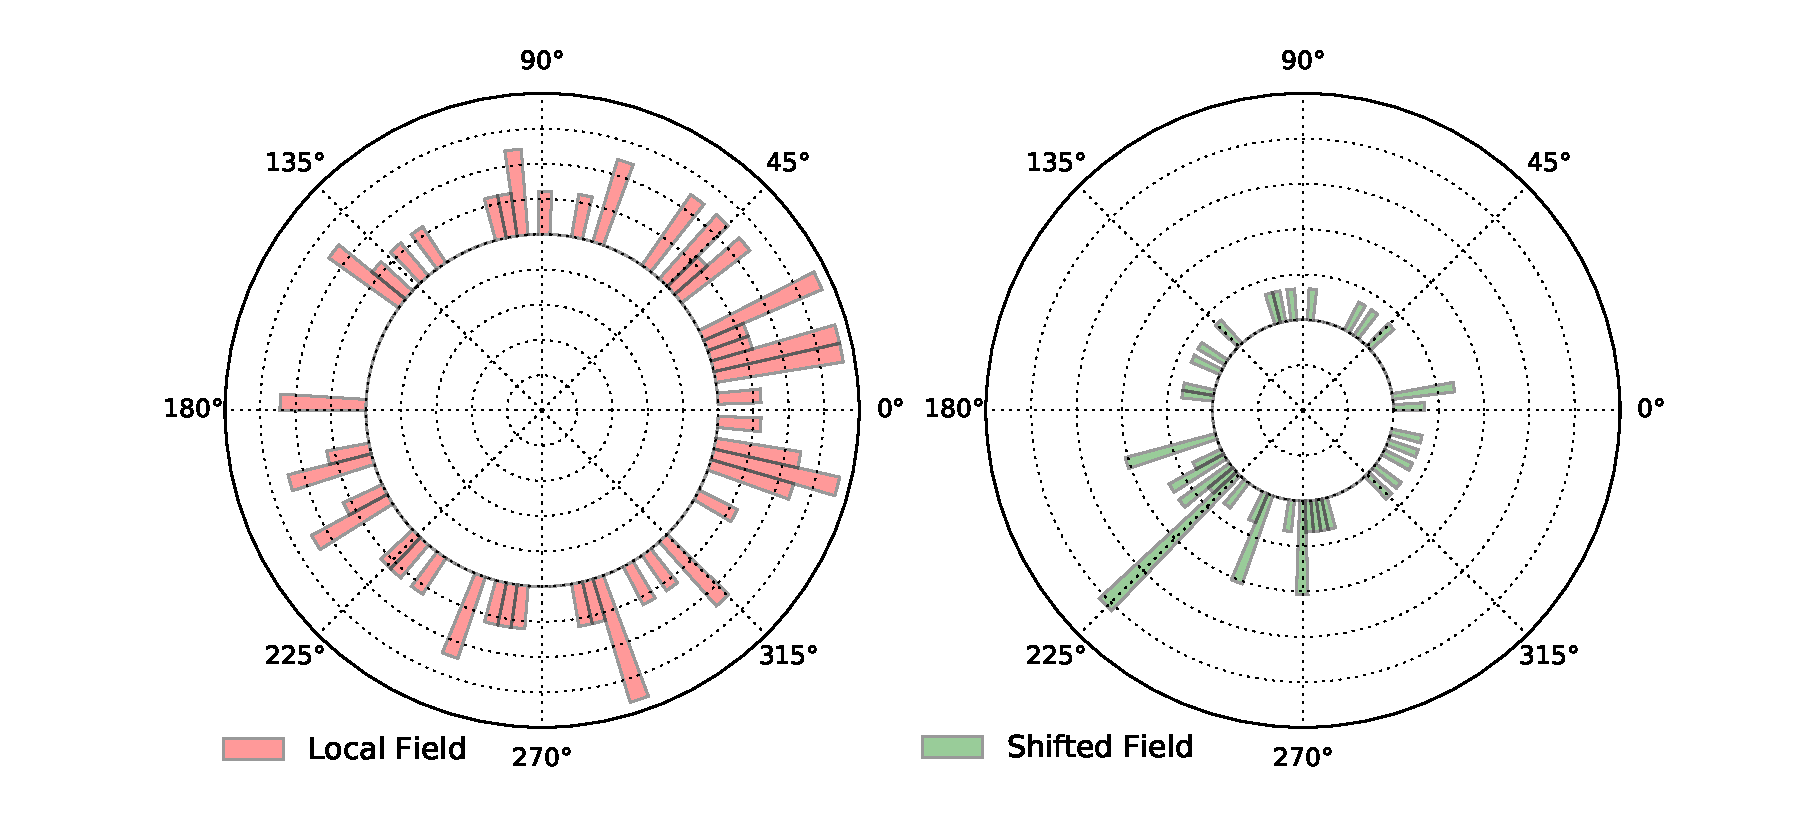
\includegraphics[width=\textwidth]{../figures/histogram}
\caption{Spatial histogram of the \texttt{orientation} of birds from the
  \texttt{swallows} population, when the magnetic field (ie \texttt{treatment}
  variable) was local (left figure) and shifted (right figure). The objective
  of the original study \cite{Giunchi2004} was to determine if swallows can
  use magnetic information for compass orientation.}
\label{fig:histogram}
\end{figure}

\subsection{Univariate Density Estimation}

The \texttt{orientation} variable is \texttt{CIRCULAR} and takes values in the
set $[0, 2\pi)$. One of the most common strategies in statistics is to approximate
the distribution of variables using a normal distribution.

\begin{minted}
[bgcolor=bg,framesep=2mm,baselinestretch=1.2,fontsize=\footnotesize,linenos]{sql}
CREATE GPM ort-norm FOR swallows USING normal(
    GENERATE (orientation)
    PROGRAM (prior nig-normal, hyperparameters learn))
INITIALIZE 6 INSTANCES OF ort-norm
INCORPORATE INTO ort-norm OBSERVATIONS (SELECT orientation FROM swallows)
ANALYZE ort-norm (TIME = 100s)
\end{minted}

The \texttt{normal} GPM type is instructed to use a collapsed normal-inverse-
gamma (NIG) normal prior on its parameters $(\mu,\sigma^2)$, and perform hyper-
parameter inference. Initializing multiple models is advantageous because
learning hyper-parameters can be done only approximately.

Evaluating the posterior distribution after \texttt{ANALYZE} can be achieved
using a BQL query. Refer to the left plot in Figure \ref{fig:normal-densities}
for the output of the \texttt{PLOT} command.

\begin{minted}
[bgcolor=bg,framesep=2mm,baselinestretch=1.2,fontsize=\footnotesize,linenos]{sql}
CREATE TABLE xvalues AS LINSPACE(0, 6.28, 100)
PLOT(xvalues, ESTIMATE PROBABILITY OF orientation = xvalues FROM ort-norm)
\end{minted}

An important point to note is that since the measurements in the dummy table
\texttt{xvalues} have primary keys that do not correspond to any previously
incorporated measurement (from the \texttt{swallows} population), the
\texttt{PROBABILITY OF} BQL queries are evaluated assuming unobserved members.

A particular issue with the GPM shown in Figure \ref{fig:normal-densities}
is that probability mass is assigned to points outside the interval $[0,2\pi)$,
effectively ignoring knowledge that \texttt{orientation} is \texttt{CIRCULAR}
and takes values on a bounded interval.

Persisting with assumption of normality, this information can be treated as a
\textit{conditioning event}, a programmatic command that the \texttt{normal}
GPM supports by specifying a \textit{truncation interval}\footnote{This GPM is
implemented fully in \texttt{gpmcc}, although conjugacy is lost due to the
truncation and inference is slower.}. By using \texttt{UPDATE SCHEMA}, all
previous incorporated measurements are maintained.

\begin{minted}
[bgcolor=bg,framesep=2mm,baselinestretch=1.2,fontsize=\footnotesize,linenos]{sql}
UPDATE SCHEMA FOR ort-norm(
    truncate (0, 6.28))
ANALYZE ort-norm (TIME = 100s)
\end{minted}

The same BQL query can be reused for visual comparison of the effect of the new
modeling command on the posterior density, as shown in Figure
\ref{fig:normal-densities}.

\begin{minted}
[bgcolor=bg,framesep=2mm,baselinestretch=1.2,fontsize=\footnotesize,linenos]{sql}
PLOT(xvalues, ESTIMATE PROBABILITY OF orientation = xvalues FROM ort-norm)
\end{minted}

\begin{figure}[H]
\centering
\begin{subfigure}[t]{.45\textwidth}
  \centering
  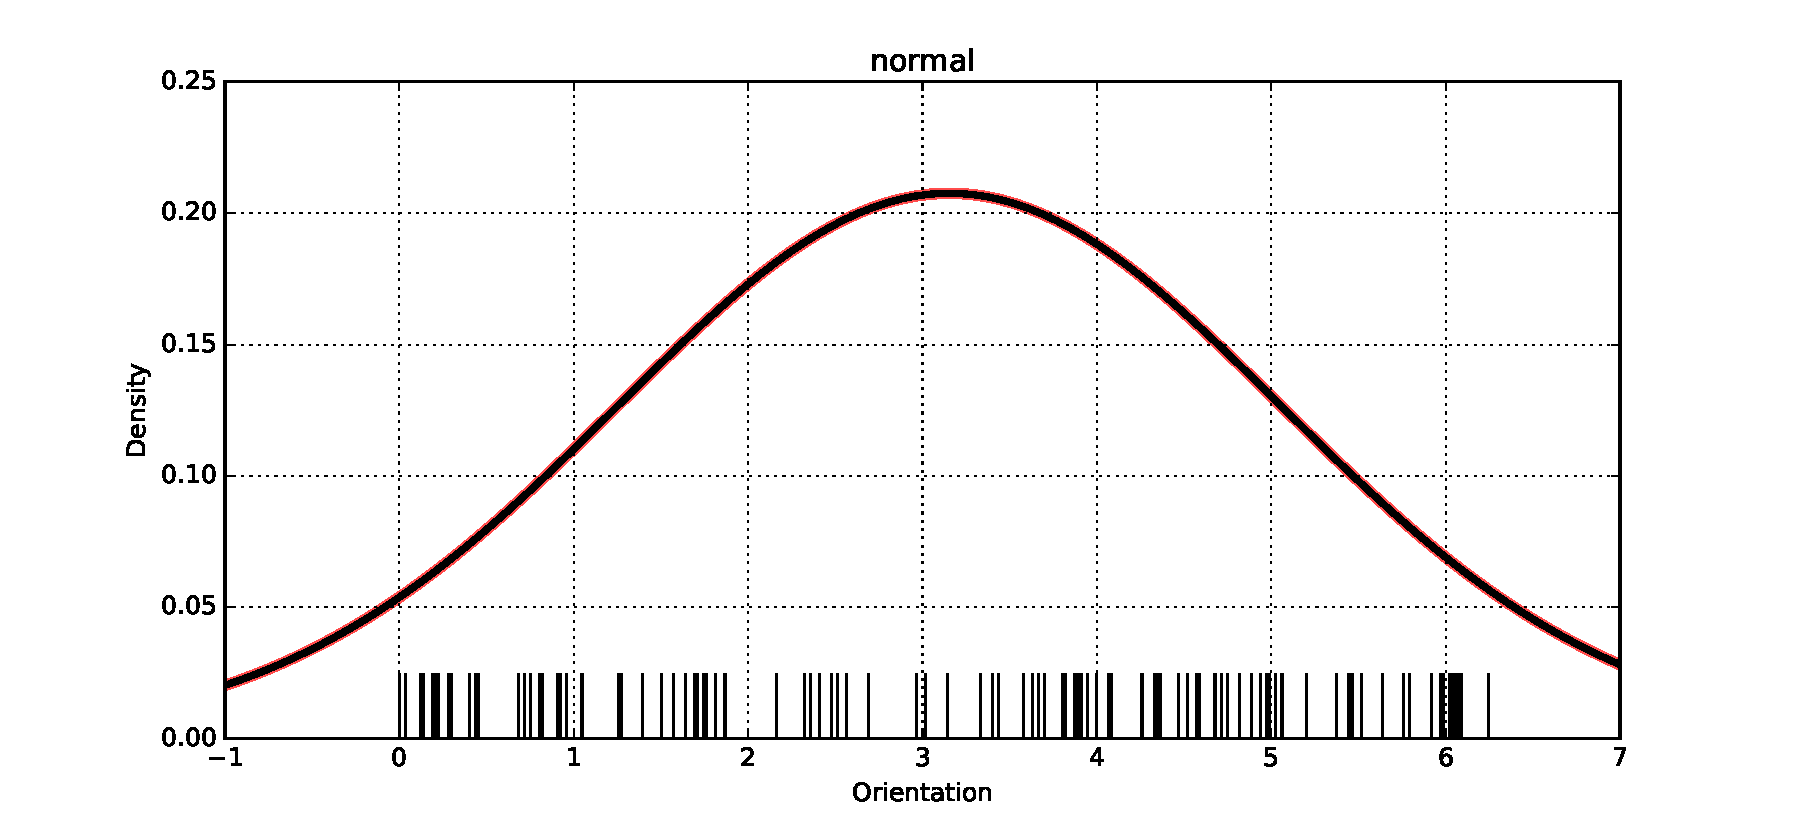
\includegraphics[width=\linewidth]{../figures/normal-density}
\end{subfigure}
\begin{subfigure}[t]{0.45\textwidth}
  \centering
  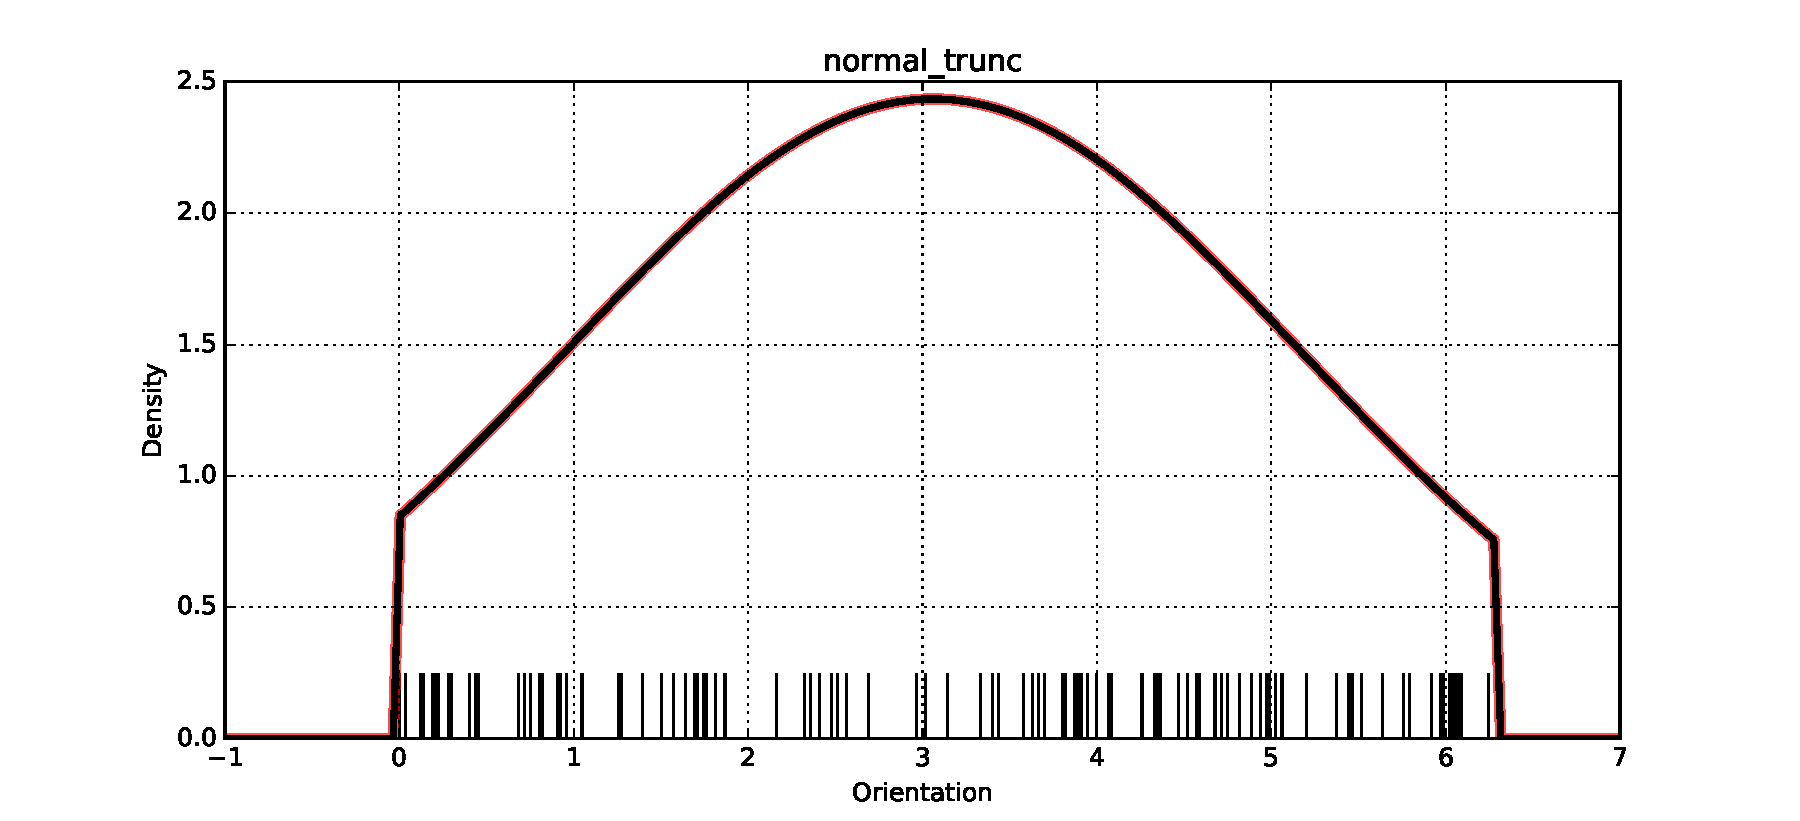
\includegraphics[width=\linewidth]{../figures/normal-trunc-density}
\end{subfigure}
\caption{Posterior distribution over \texttt{orientation} learned by the
    \texttt{ort-norm} GPM before (left) and after (right) updating its schema
    with \texttt{truncate(0, 6.28)}. Observe the value of the posterior
    density on the y-axis increases by a factor of 10, as probability
    mass is reassigned to the interval.}
\label{fig:normal-densities}
\end{figure}

\subsection{Mixture Modeling of Univariate Densities}

Both plots in Figure \ref{fig:normal-densities} illustrate a poor fit to
the data, which can be seen visually. There are many samples at the edges of the
interval, and only a few samples in the center. However the posterior mode of
the \texttt{ort-norm} GPM is forced to the center, and assigns low density to
high density regions and vice versa.

To deal with the perceived \textit{multi-modality}, one can \textit{compose}
many instances of the truncated \texttt{normal} GPM by creating a
\texttt{dp-mixture} GPM.

\begin{minted}
[bgcolor=bg,framesep=2mm,baselinestretch=1.2,fontsize=\footnotesize,linenos]{sql}
CREATE GPM ort-norm-mixture FOR swallows USING dp-mixture(
    GENERATE (orientation)
    PROGRAM (
        MODEL orientation AS normal
            (prior nig-normal, hyperparameters learn)))

INITIALIZE 2 INSTANCES OF ort-norm-mixture
INCORPORATE INTO ort-norm-mixture OBSERVATIONS (SELECT orientation FROM swallows)
ANALYZE ort-norm-mixture (
    TRANSITION ALL
    ITERATIONS = 100)
\end{minted}

The \texttt{PROGRAM} of a \texttt{dp-mixture} instructs to use the
\texttt{normal} GPM as the parametric family to mix, with a NIG-normal base
measure. Any other commands accepted by the \texttt{normal} GPM, such as the
truncation range can be used as well. In general, the current implementation of
\texttt{dp-mixture} allows composition any GPMs which are univariate (one
\texttt{GENERATE}) and unconditional (no \texttt{GIVENS}). Moreover, the GPMs
must be of the same \textit{type}. A GPM which relaxes these constraint will be
encountered shortly.

Observe that the program in \texttt{ANALYZE} contains the directive
\texttt{TRANSITION ALL}, which tell to Gibbs cycle through \textbf{all} its
inference kernels, (row assignments, uncollapsed column parameters, column hyper-
parameters, CRP $\alpha$), for 100 sweeps.

As before, the same BQL query can be used for visual evaluation. However, this
time individual models are targeted (specified by \texttt{USING MODEL n}),
rather than aggregating (the default behavior). This query allows visualization
of the degree of agreement between independent GPM instances of
\texttt{ort-norm-mixture}.

\begin{minted}
[bgcolor=bg,framesep=2mm,baselinestretch=1.2,fontsize=\footnotesize,linenos]{sql}
PLOT(xvalues, ESTIMATE PROBABILITY OF orientation = xvalues FROM ort-norm-mixture
    USING MODEL 1)
PLOT(xvalues, ESTIMATE PROBABILITY OF orientation = xvalues FROM ort-norm-mixture
    USING MODEL 2)
\end{minted}

\begin{figure}[H]
\centering
\begin{subfigure}[t]{.45\textwidth}
  \centering
  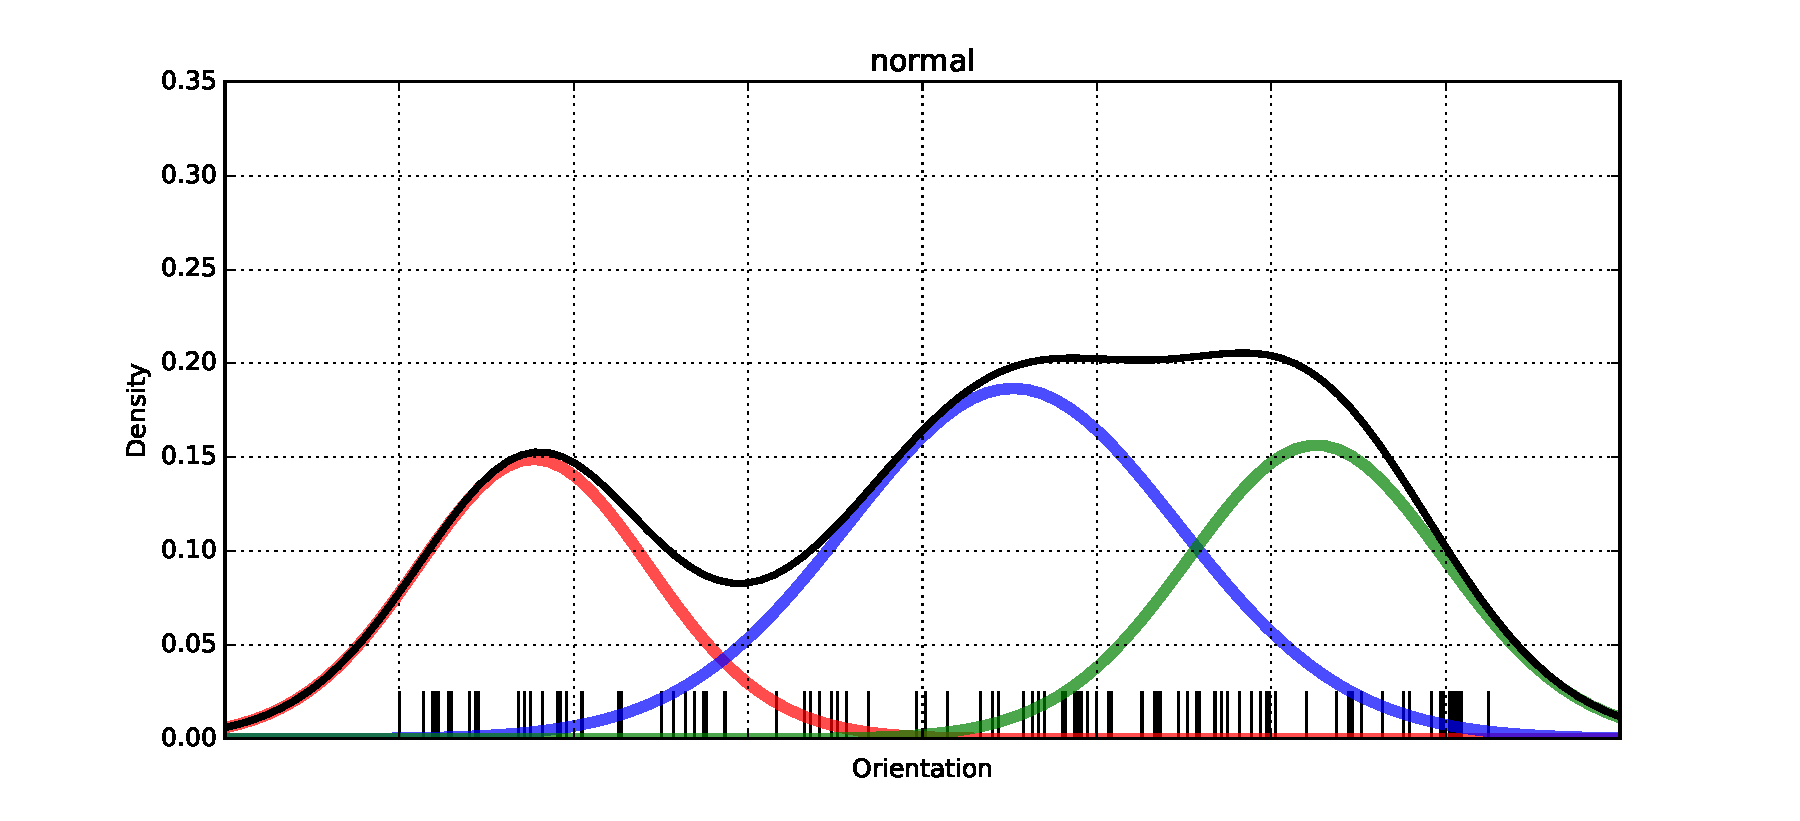
\includegraphics[width=\linewidth]{../figures/normal-mixture-density}
\end{subfigure}
\begin{subfigure}[t]{0.45\textwidth}
  \centering
  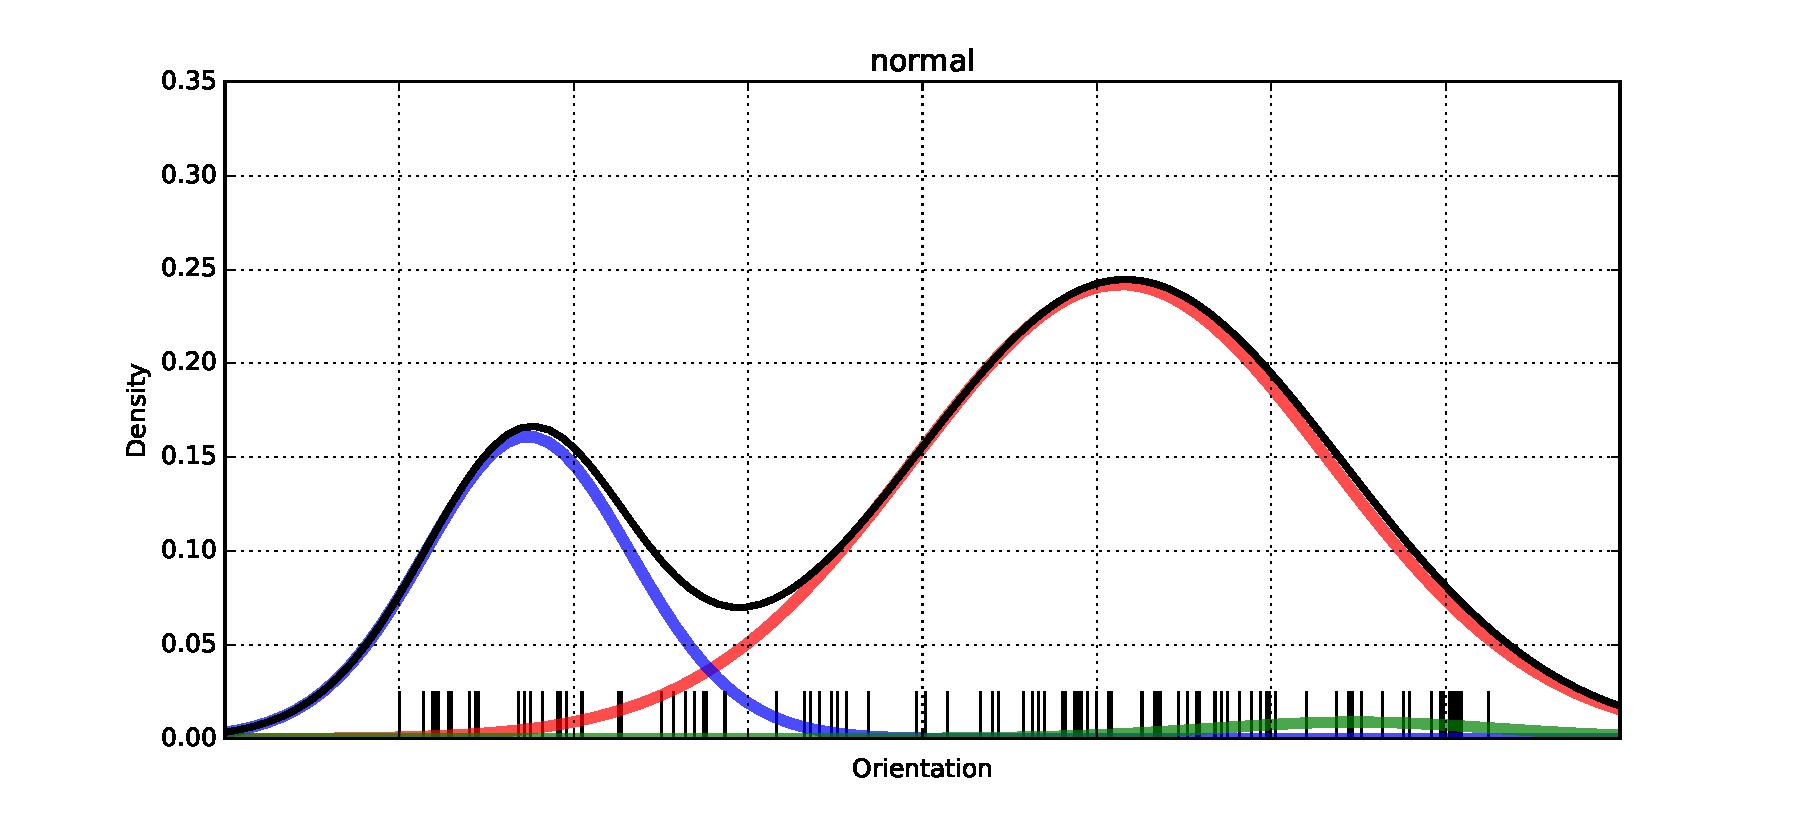
\includegraphics[width=\linewidth]{../figures/normal-mixture-density-2}
\end{subfigure}
\caption{Posterior distribution over \texttt{orientation} learned by two
independent model instances of the \texttt{ort-norm-mixture} GPM. Colored lines
represent individual instances of the \texttt{normal} GPM that live inside the
the \texttt{dp-mixture} GPM.}
\label{fig:normal-mixture-densities}
\end{figure}

\section{Beyond Normality and Density Estimation Comparison}

Three modeling approaches for the generative process for the \texttt{orientation}
variable have been explored thus far

\begin{itemize}
\item Univariate normal.
\item Univariate normal, truncated to the \texttt{CIRCULAR} range.
\item DP mixture of univariate normals, without truncation.
\end{itemize}

Are there reasons to consider other GPMs that are not normal and have properties
that better match the \texttt{orientation} variable? Consider the following
possibilities:

\begin{itemize}
\item Scaling a distribution on an arbitrary bounded interval to the circular
    interval $[0, 2\pi)$, such as the standard beta on
    $(0,1)$\footnote{Supported by gpmcc.}.

\begin{minted}
[bgcolor=bg,framesep=2mm,baselinestretch=1.2,fontsize=\footnotesize,linenos]{sql}
CREATE GPM ort-beta-mixture FOR swallows USING dp-mixture(
    GENERATE (orientation)
    PROGRAM (
        MODEL orientation AS beta
            (scale(0, 2pi), hyperparameters fixed)))
\end{minted}

\item Using a distribution especially appropriate for the \texttt{CIRUCLAR}
measurement type, such as the Vonmises distribution\footnote{Available in
gpmcc.}.

\begin{minted}
[bgcolor=bg,framesep=2mm,baselinestretch=1.2,fontsize=\footnotesize,linenos]{sql}
CREATE GPM ort-vonmises FOR swallows USING vonmises(
    GENERATE (orientation))
\end{minted}
\end{itemize}

A common metric, highly flawed, for evaluating the performance of density
estimators is segregating data into a \textit{training} set and \textit{testing}
set, incorporating and runing analysis on the training set, and then evaluating
the \textit{predictive likelihood} on the \textit{test set}. A more Bayesian
approach is to observe all the data and then try to compute the
\textit{marginal likelihood} of the measurements after analysis. The following
program illustrates how MML and BQL can be used to compare these metrics for the
four GPMs \texttt {ort-normal-mixture}, \texttt{ort-trunc-mixture},
\texttt{ort-beta-mixture}, and \texttt{ort-vonmises}, assuming they have been
\texttt{CREATED} and \texttt{INITIALIZED} with 28 instances each.

The square brackets with multiple GPM names are constructs permitted by MML and
BQL, and are syntactic sugar for repeating the same directive or query for
each GPM in the list.

\begin{minted}
[bgcolor=bg,framesep=2mm,baselinestretch=1.2,fontsize=\footnotesize,linenos]{sql}
-- Use first 80 observations for the training set.
INCORPORATE INTO [ort-norm-mixture | ort-trunc-mixture | ort-beta-mixture |
    ort-vonmises] OBSERVATIONS (SELECT orientation FROM swallows WHERE pk <= 80)
-- Allow 100 seconds of analysis.
ANALYZE [ort-norm-mixture | ort-trunc-mixture | ort-beta-mixture | ort-vonmises
    (TIMEOUT=100s)
-- Evaluate predictive likelihood on 20 training samples.
ESTIMATE PROBABILITY OF orientation =
    (SELECT orientation FROM swallows WHERE pk BETWEEN (80, 100))
    FROM [ort-norm-mixture | ort-trunc-mixture | ort-beta-mixture | ort-vonmises]
-- Evaluate the marginal likelihood.
ESTIMATE MARGINAL LIKELIHOOD FROM
    [ort-norm-mixture | ort-trunc-mixture | ort-beta-mixture | ort-vonmises]
\end{minted}


\begin{figure}[H]
\centering
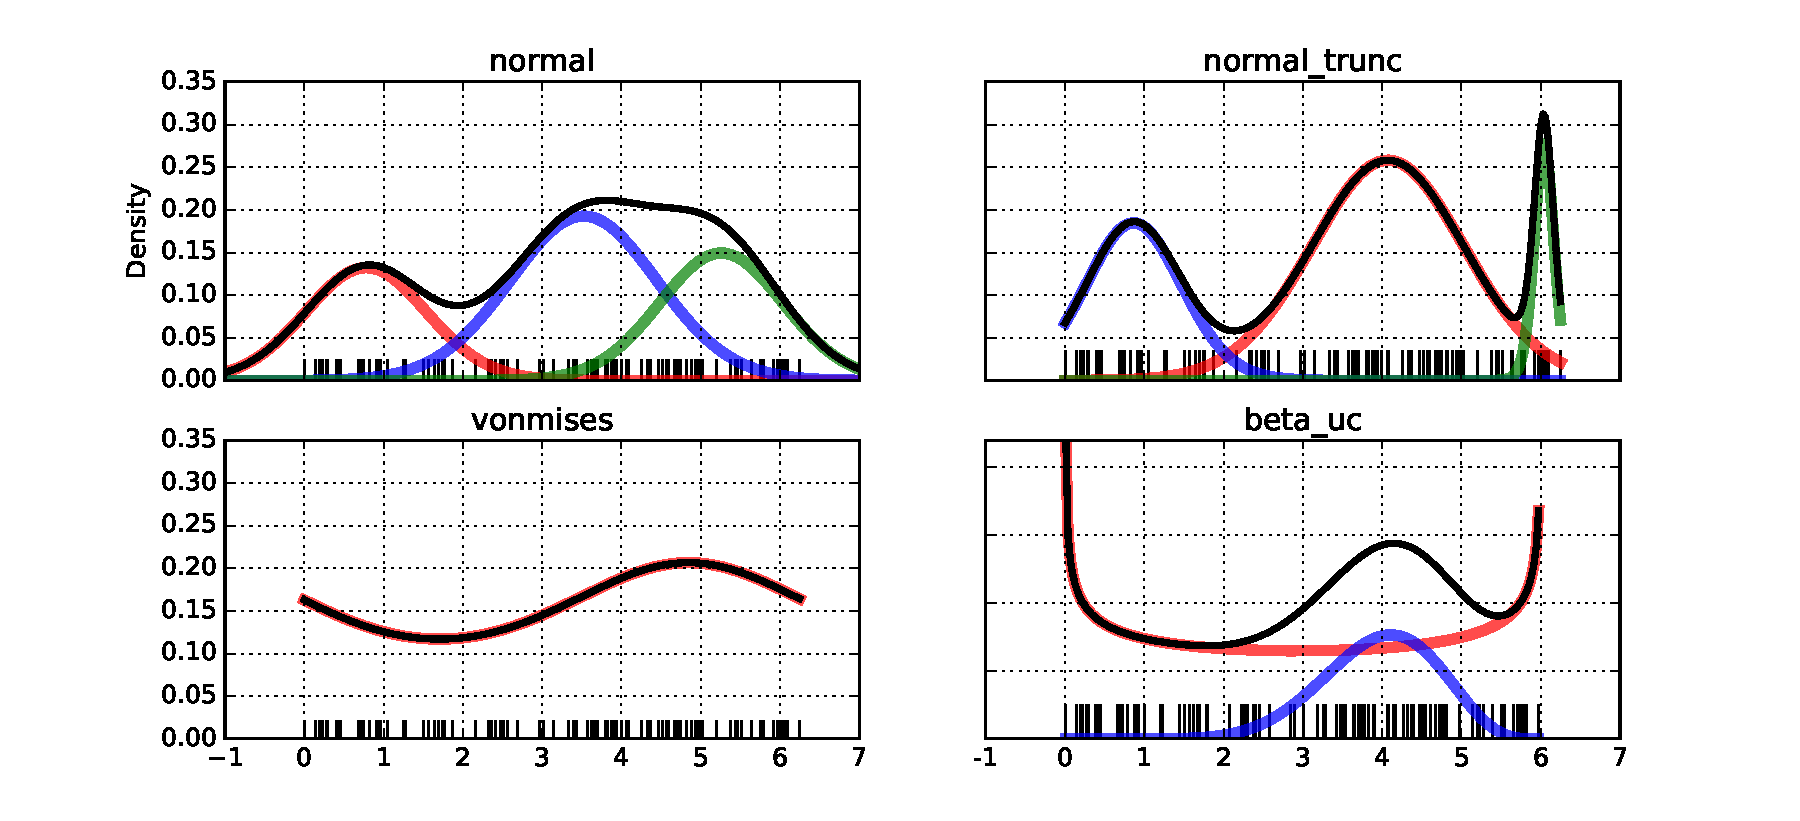
\includegraphics[width=.7\linewidth]{../figures/mixtures}
\caption{Samples from the posterior distribution over \texttt{orientation}
learned by the four competing GPMs Only the \texttt{vonmises} is a single
univariate estimator, while the others are \texttt{dp-mixture} of their
respective densities.}
\label{fig:predictive-comparisons}
\end{figure}

\begin{figure}[H]
\centering
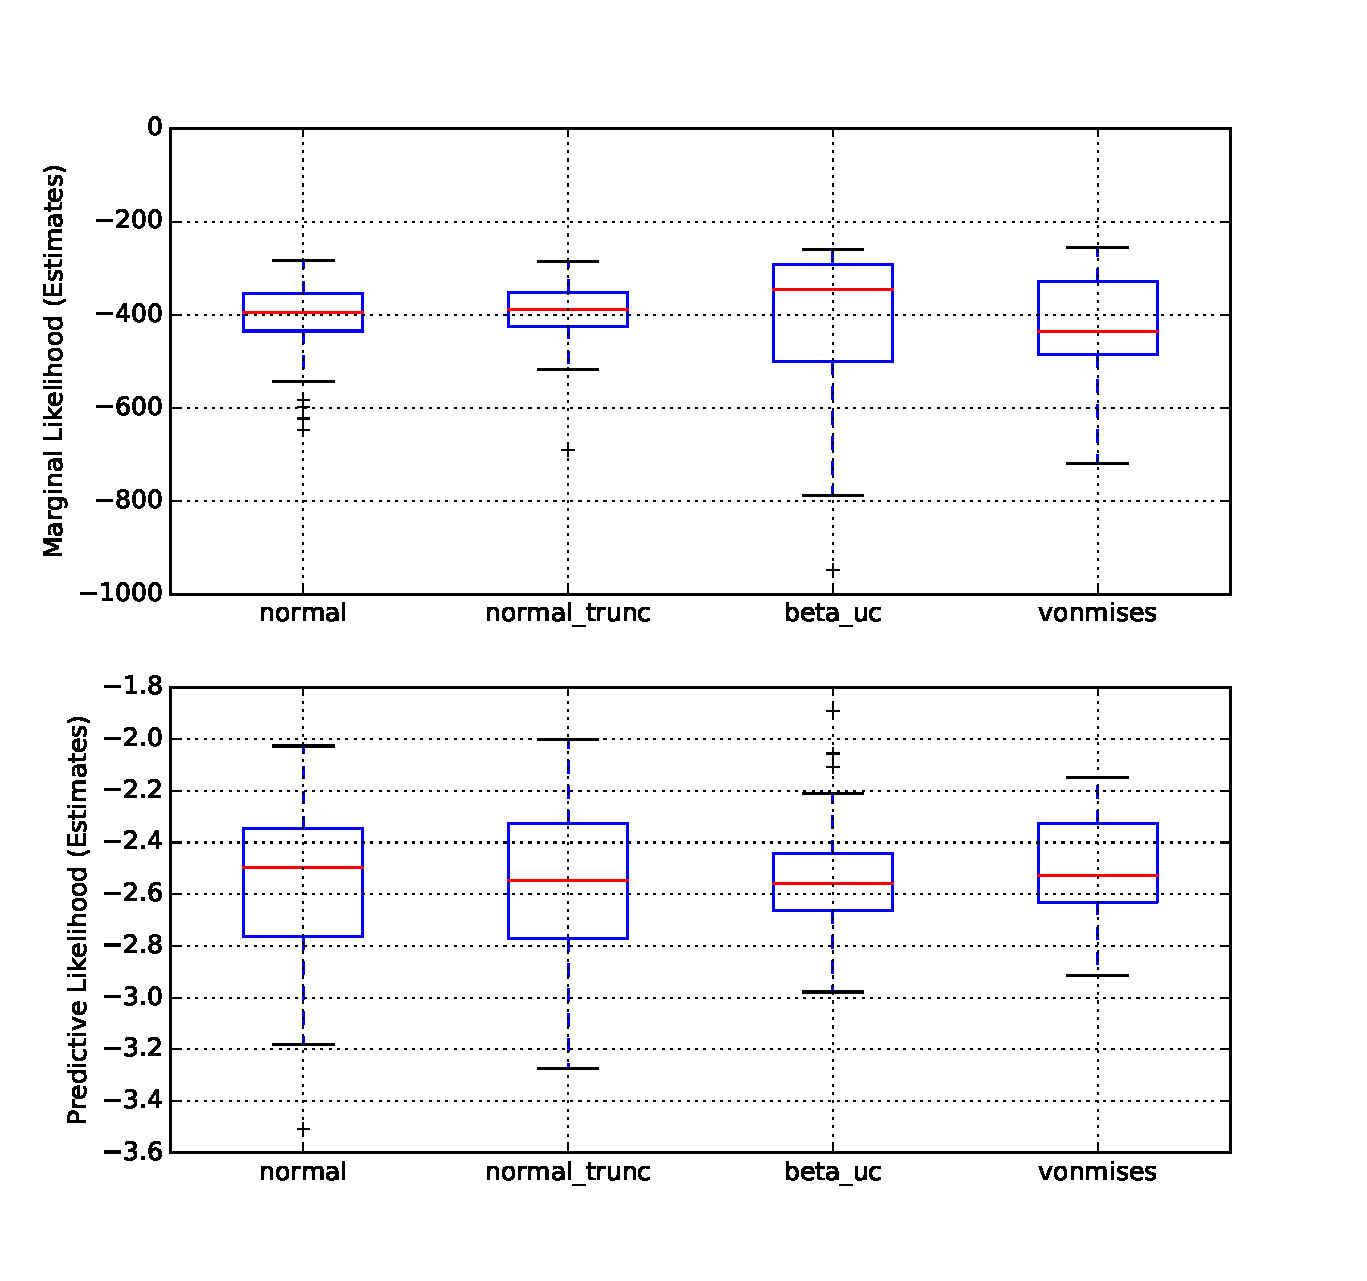
\includegraphics[width=.5\linewidth]{../figures/boxplots}
\caption{Distribution of estimates of the marginal likelihood (top) and
predictive likelihood (bottom) on the held out test set. Uncertainty over the
predictive likelihood is over the test samples. Uncertainty in the marginal
likelihood is over the 28 individual models in each ensemble GPM. Surprisingly,
there does not appear to be major differences in the GPM performance using
either of these two metrics.}
\label{fig:boxplots}
\end{figure}

\section{Learning Joint Distributions And Evaluating Classification Performance
Using a GPM}

Recall that the \texttt{swallows} population contains the two variables
\texttt{treatment} and \texttt{orientation}. So far, these two variables have
been modeled separately. The \texttt{crosscat} GPM is a generalization of
\texttt{dp-mixture} for multiple \texttt{GIVEN} variables.

\begin{minted}
[bgcolor=bg,framesep=2mm,baselinestretch=1.2,fontsize=\footnotesize,linenos]{sql}
CREATE GPM swallows-crosscat FOR swallows USING crosscat(
    GENERATE (treatment, orientation)
    PROGRAM (
        MODEL treatment AS bernoulli
        MODEL orientation AS normal))
\end{minted}

One method to measure how well \texttt{swallows-crosscat} has learned the joint
distribution is to ask the GPM to classify unseen \texttt{orientation}
measurements into either \textit{local} or \textit{shifted}
\texttt{treatment}\footnote{It should
be noted that this task is very difficult (see Figure \ref{fig:histogram}) and
is included only for illustrative purposes.}. The following MML code sets
up and runs the experiment in BQL.

\begin{minted}
[bgcolor=bg,framesep=2mm,baselinestretch=1.2,fontsize=\footnotesize,linenos]{sql}
-- Split the population.
CREATE POPULATION swallows-train AS (SELECT * FROM SWALLOWS LIMIT 80)
CREATE POPULATION swallows-test AS (SELECT * FROM SWALLOWS WHERE pk BEWTEEN (80, 100))
-- Incorporate.
INCORPORATE INTO swallows-crosscat
    OBSERVATIONS swallows-train
-- Analyze.
ANALYZE swallows-crosscat (TIMEOUT 100s)
-- Obtain probability of treatment = local for orientations in the test set.
CREATE POPULATION soft-predictions AS
    ESTIMATE PROBABILITY OF (treatment = 'local')
            GIVEN orientation = (SELECT orientation FROM swallows-test) FROM swallows-crosscat
-- Use a hard classification rule with a threshold of 0.5.
CREATE POPULATION hard-predictions AS
    SELECT (treatment FROM swallows-test) AS true-labels,
    CASE WHEN prob-of-local > 0.5 THEN 'local' ELSE 'shifted' END
        AS predicted-labels
    FROM soft-predictions
\end{minted}

The population \texttt{hard-predictions} now contains a 0-1 prediction for
\texttt{treatment} on all measurements in the test set. There are many metrics
for evaluating binary classification. It was in proposed in \cite{Wallach2006}
that the \textit{mutual information} between true labels and predictions is a
metric with desirable properties. A new GPM, called
\texttt{classification-evaluation} based on the \texttt{frequency} GPM is ideal
for computing this metric.

\begin{minted}
[bgcolor=bg,framesep=2mm,baselinestretch=1.2,fontsize=\footnotesize,linenos]{sql}
-- Create the GPM for evaluating classification
CREATE GPM classification-evaluator FOR hard-predictions USING frequency(
    GENERATE (true-labels, predicted-labels))
INCORPORATE INTO classification-evaluator OBSERVATIONS hard-predictions
ANALYZE classification-evaluator
-- Compute the mutual information of labels and predictions.
ESTIMATE MUTUAL INFORMATION of true-labels, predicted-labels FROM classification-evaluator
\end{minted}

To visualize the results, the experiment above was implemented for four GPMs
based on \texttt{crosscat} using different internal GPMs for
\texttt{orientation} (\texttt{normal}, \texttt{normal-trunc} \texttt{vonmises}
and \texttt{beta}) for various thresholds. Figure
\ref{fig:mutual-information} summarizes the results of this experiment.

\begin{figure}[H]
\centering
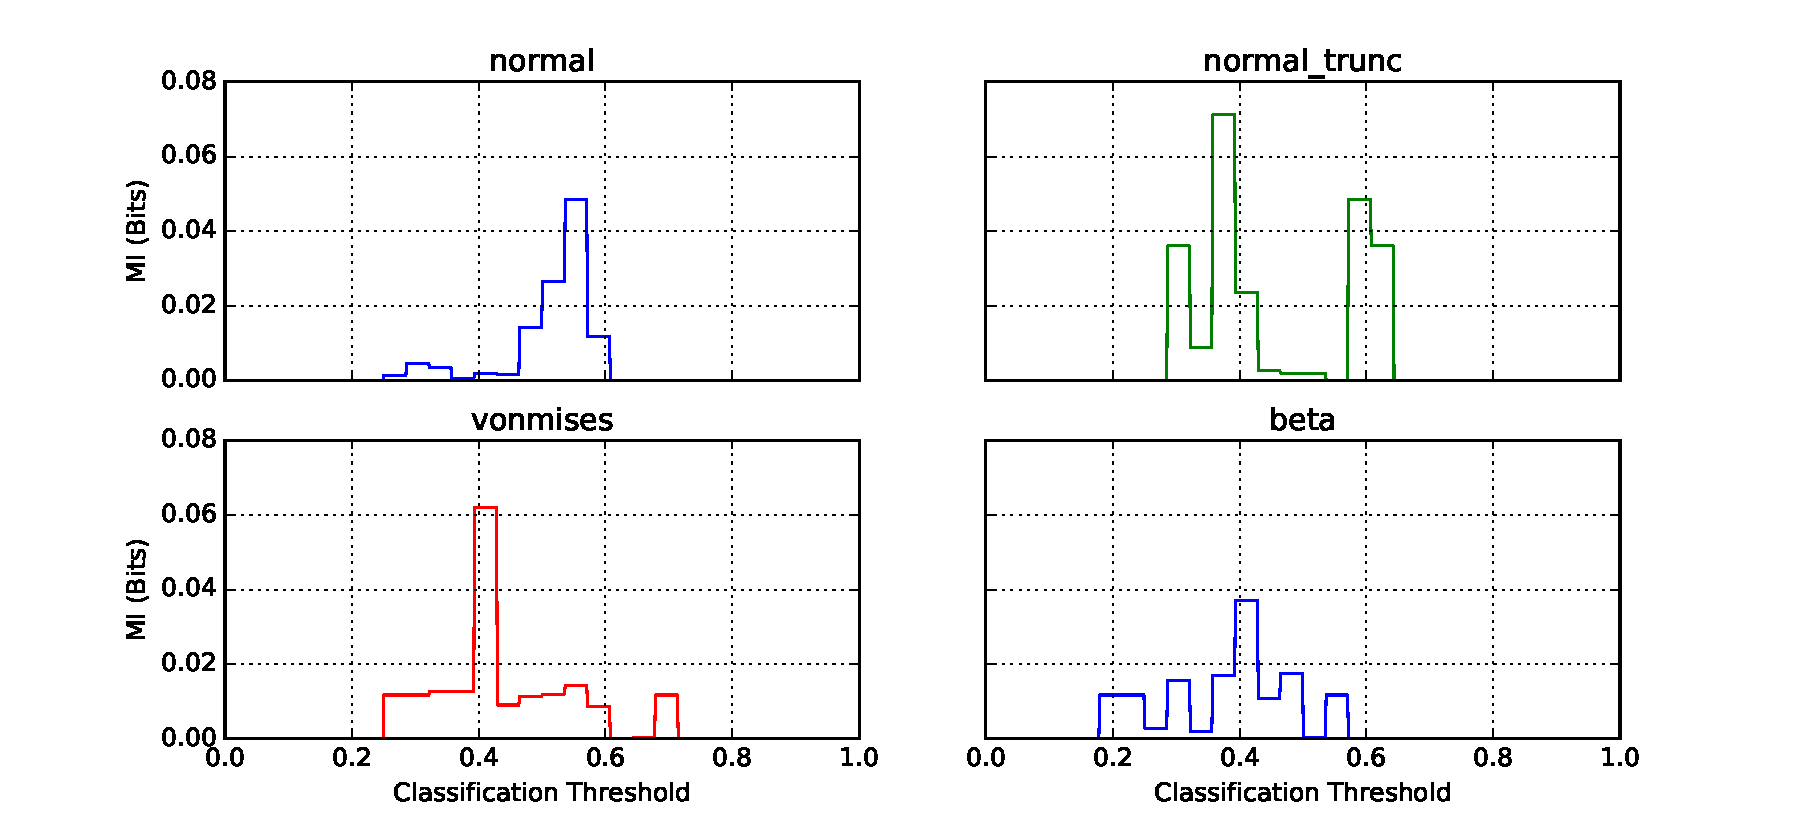
\includegraphics[width=.8\linewidth]{../figures/mutual-information}
\caption{Mutual information of true labels and predicted labels of
\texttt{treatment} computed by the \texttt{classification-evaluator} GPM. The
test set has 20 observations, and the classification threshold varies between
0 and 1 in increments of .1. The title of each subplot shows the GPM that
\texttt{crosscat} was instructed to use to model the \texttt{orientation}
variable. No error bars are shown since only one was test-train split was used.}
\label{fig:mutual-information}
\end{figure}

\section{Todo}

\begin{itemize}
\item Introduce some discriminative models (not density estimators) such as SVM,
regression, etc as standalone GPMs.
\item Discuss how this MML version easily allows for computationally derived
column to be added, modeled, etc with an example.
\item Introduce crosscat.
\item Introduce compositor network and its CMML language.
\item Explain the formalism of hybrid probabilistic-discriminative models
    \subitem Unlocalized (imputation only).
    \subitem Explicitly localized (no feedback from discriminative to
        generative GPM).
    \subitem Implicitly localized (fully feedback from discriminative
        to generative GPM).
\end{itemize}

\bibliographystyle{alpha}
\bibliography{writeup}
\end{document}
